\documentclass[10pt, a4paper,spanish]{article}
\usepackage[utf8]{inputenc}

\usepackage{varwidth}
\usepackage{graphicx}

\usepackage[T1]{fontenc} % Use 8-bit encoding that has 256 glyphs
\usepackage{microtype} % Slightly tweak font spacing for aesthetics

\usepackage[hmarginratio=1:1,top=32mm,columnsep=20pt]{geometry} % Document margins
\usepackage[hang, small,labelfont=bf,up,textfont=it,up]{caption} % Custom captions under/above floats in tables or figures
\usepackage{float} % Required for tables and figures in the multi-column environment - they need to be placed in specific locations with the [H] (e.g. \begin{table}[H])
\usepackage{hyperref} % For hyperlinks in the PDF

\usepackage{abstract} % Allows abstract customization
\renewcommand{\abstractnamefont}{\normalfont\bfseries} % Set the "Abstract" text to bold
\renewcommand{\abstracttextfont}{\normalfont\small\itshape} % Set the abstract itself to small italic text

\usepackage{titlesec} % Allows customization of titles
\renewcommand\thesection{\Roman{section}} % Roman numerals for the sections
\renewcommand\thesubsection{\Roman{subsection}} % Roman numerals for subsections
\titleformat{\section}[block]{\large\scshape\centering}{\thesection.}{1em}{} % Change the look of the section titles
\titleformat{\subsection}[block]{\large}{\thesubsection.}{1em}{} % Change the look of the section titles

\usepackage{fancyhdr} % Headers and footers
\pagestyle{fancy} % All pages have headers and footers
\fancyhead{} % Blank out the default header
\fancyfoot{} % Blank out the default footer
\fancyhead[C]{ Marzo 2016 $\bullet$ JumpVa $\bullet$ Análisis de la Aplicación} % Custom header text
\fancyfoot[RO,LE]{\thepage} % Custom footer text

%----------------------------------------------------------------------------------------
%	TITLE SECTION
%----------------------------------------------------------------------------------------

\title{\vspace{-15mm}\fontsize{24pt}{10pt}\selectfont\textbf{Análisis de la Aplicación}} % Article title

\author{
\large
\textsc{Alberto Amigo Alonso\textsubscript{25\%}}\\[2mm] % Your name
\textsc{Sergio Delgado Álvarez\textsubscript{25\%}}\\[2mm] % Your name
\textsc{Sergio García Prado\textsubscript{25\%}}\\[2mm] % Your name
\textsc{Oscar Fernández Angulo\textsubscript{25\%}}\\[2mm] % Your name
\normalsize Universidad de Valladolid \\ % Your institution
\vspace{-5mm}
}
\date{}

%----------------------------------------------------------------------------------------

\begin{document}

	\maketitle % Insert title

	\thispagestyle{fancy} % All pages have headers and footers

%----------------------------------------------------------------------------------------
%	ABSTRACT
%----------------------------------------------------------------------------------------

	\begin{abstract}
		\noindent Servicio web destinado a permitir a remitentes y destinatarios ofertar envíos para que los transportistas sean capaces de encontrarlos permitiendo a todos los usuarios monitorizarlos.
	\end{abstract}

%----------------------------------------------------------------------------------------
%	TEXT
%----------------------------------------------------------------------------------------
	\section{Especificación de requisitos:}

		\paragraph{}
		Requisitos funcionales: El sistema deberá...

			\begin{itemize}
				\item registrar nuevos usuarios.
				\item reconocer el rol de cada usuario.
				\item crear un nuevo envío.
				\item buscar un envío en su historial.
				\item cambiar el estado de los envíos.
				\item permitir al usuario puntuar los envíos.
				\item guardar un historial de los envíos (información).
				\item permitir a los usuarios consultar el estado de los envíos.
				\item actualizar el progreso de los envíos.
				\item permitir a los transportistas pujar por un envío.
				\item permitir a los usuarios añadir hitos a un envío.
				\item asegurar que todos los usuarios están previamente identificados en el sistema para poder acceder a cualquier función.
				\item notificar al usuario nuevas incidencias en los envíos.
				\item permitir a "los que envían" consultar el historial de los transportistas relacionados con el envío.
				\item permitir a "los que envían" puntuar al transportista que ha realizado su envío.
				\item permitir a los transportistas realizar una oferta para un evento.
				\item pedir una confimación para realizar una oferta.
				\item pedir una confimación para asignar un envío.
				\item permitir al transportista buscar nuevos envíos.
			\end{itemize}

			\paragraph{}
			Requisitos no funcionales: El sistema deberá...

				\begin{itemize}
					\item usar una base de datos como medio de almacenamiento.
					\item permitir hacer login a los usuarios que están en la base de datos.
				\end{itemize}
	\section{Casos de uso:}


		\begin{figure}[H]
			\centering
				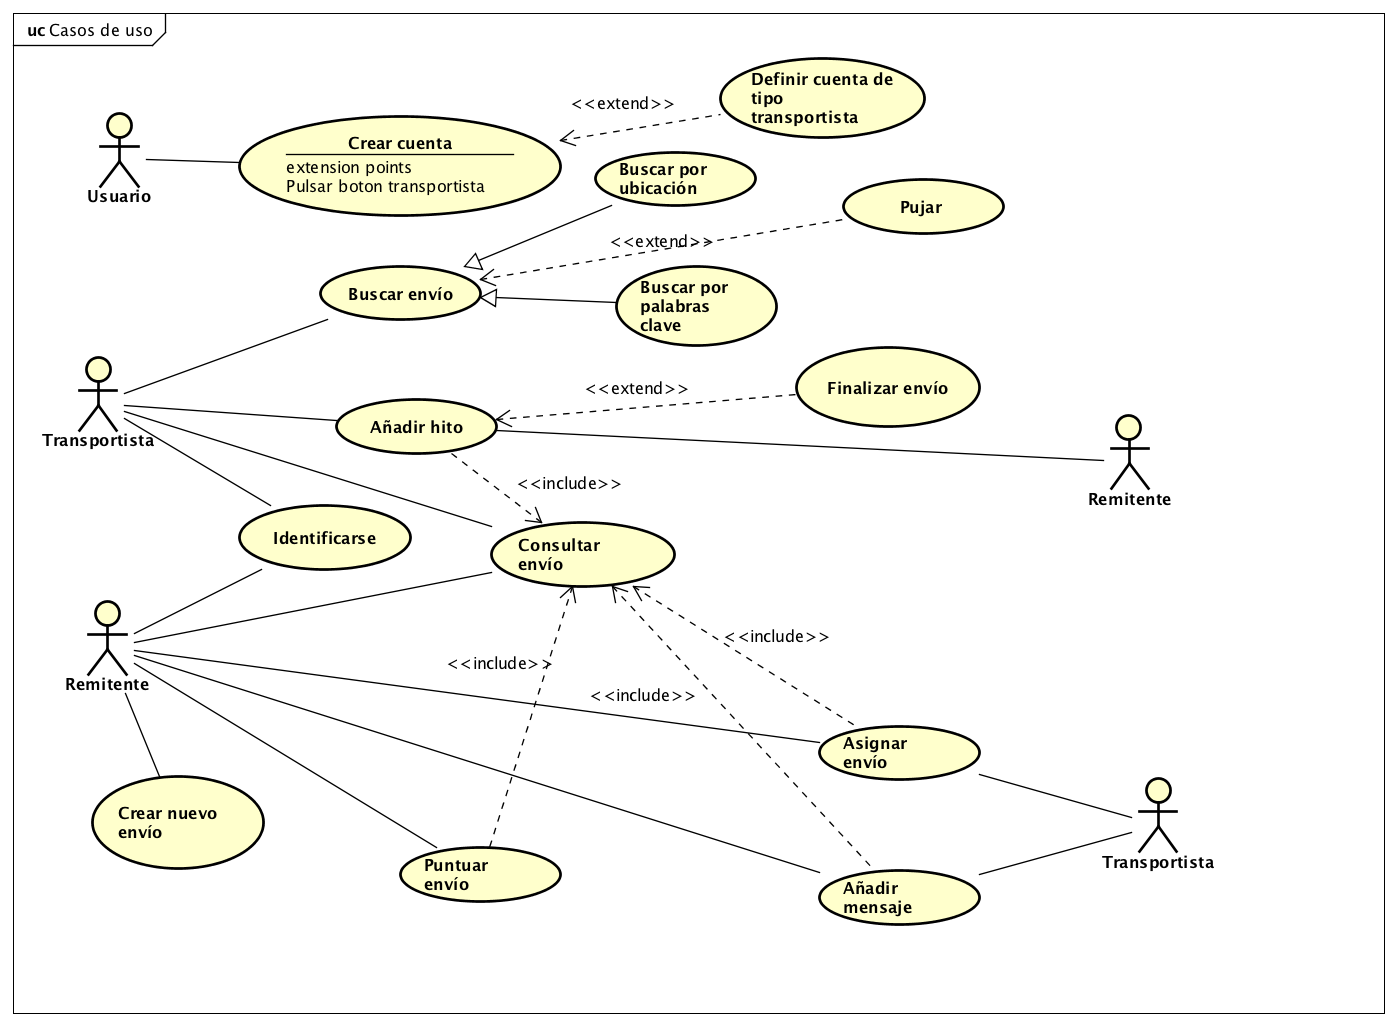
\includegraphics[width=\textwidth]{astah/casos_de_uso.png}
		\end{figure}

		\begin{figure}[H]
			\centering
				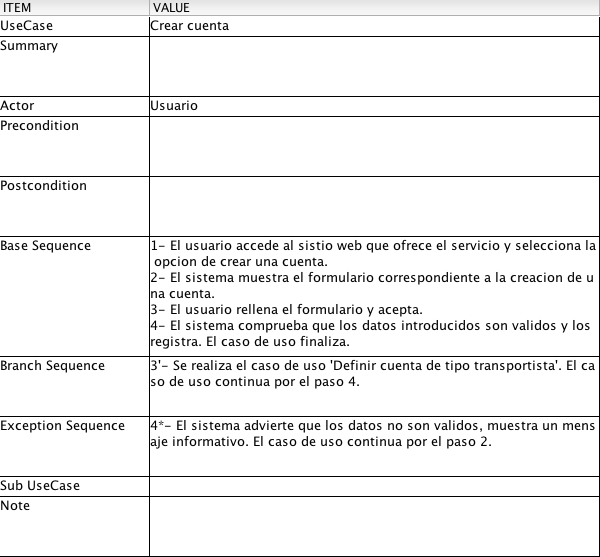
\includegraphics[width=0.75\textwidth]{astah/use_case_crear_cuenta.png}
		\end{figure}

		\begin{figure}[H]
			\centering
				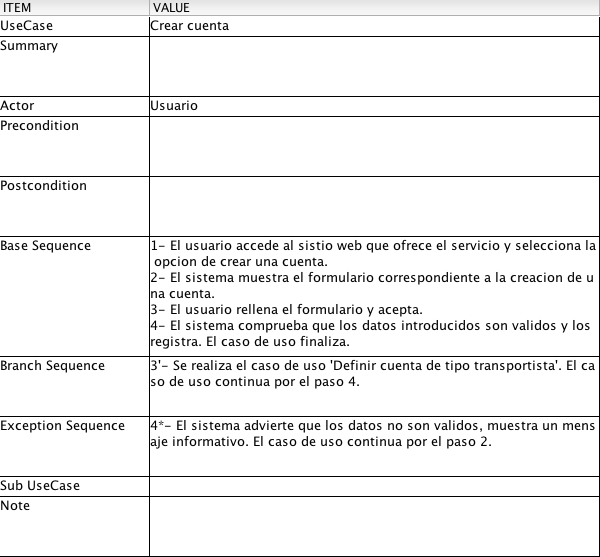
\includegraphics[width=0.75\textwidth]{astah/use_case_crear_cuenta.png}
		\end{figure}

		\begin{figure}[H]
			\centering
				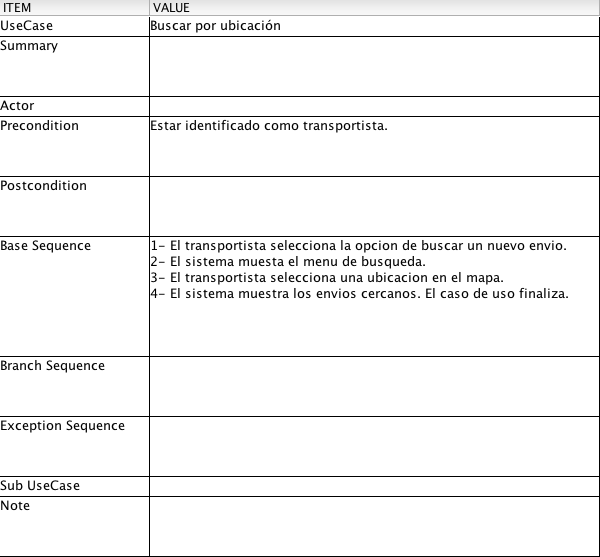
\includegraphics[width=0.75\textwidth]{astah/use_case_buscar_ubicacion.png}
		\end{figure}

		\begin{figure}[H]
			\centering
				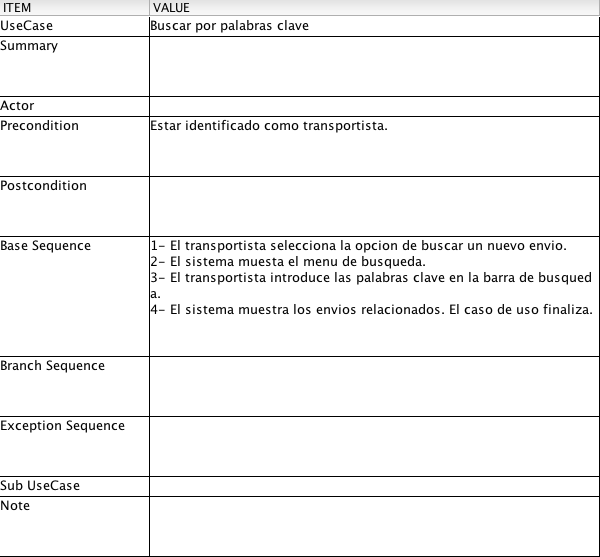
\includegraphics[width=0.75\textwidth]{astah/use_case_buscar_palabras_clave.png}
		\end{figure}

		\begin{figure}[H]
			\centering
				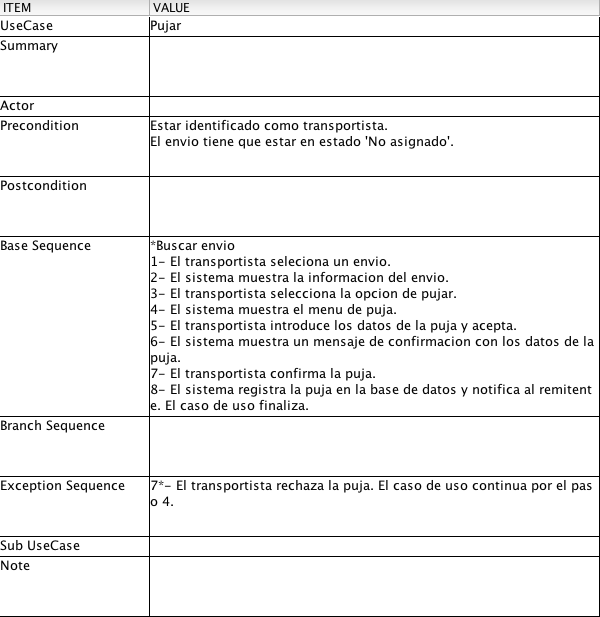
\includegraphics[width=0.75\textwidth]{astah/use_case_pujar.png}
		\end{figure}

		\begin{figure}[H]
			\centering
				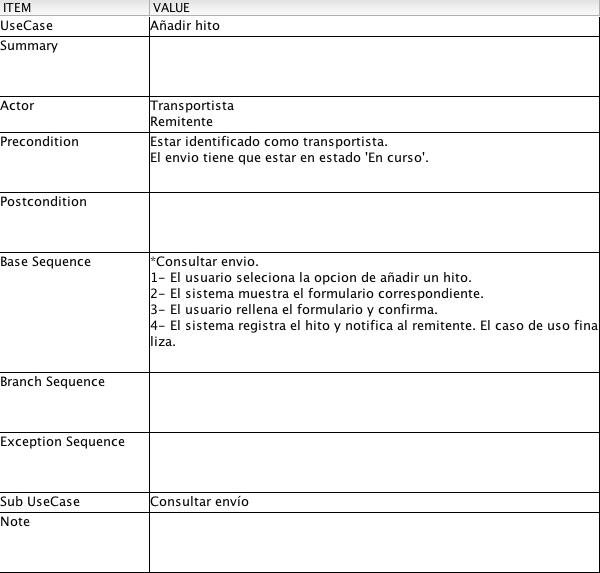
\includegraphics[width=0.75\textwidth]{astah/use_case_anadir_hito.png}
		\end{figure}

		\begin{figure}[H]
			\centering
				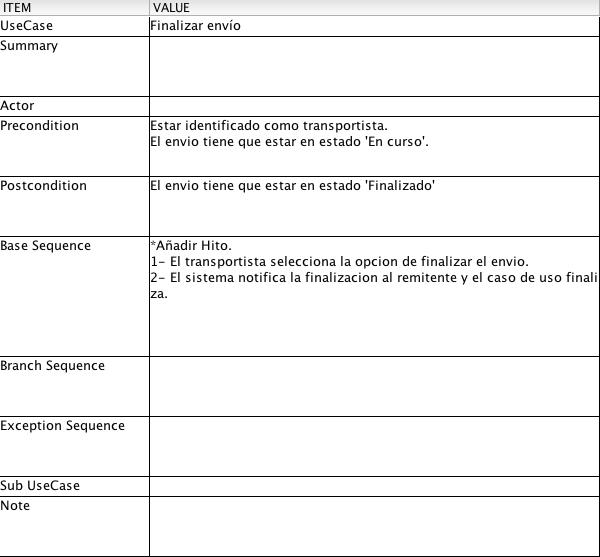
\includegraphics[width=0.75\textwidth]{astah/use_case_finalizar_envio.png}
		\end{figure}

		\begin{figure}[H]
			\centering
				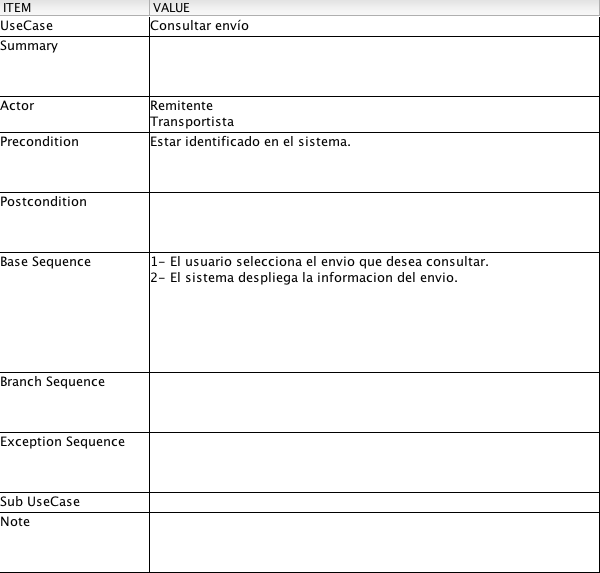
\includegraphics[width=0.75\textwidth]{astah/use_case_consultar_envio.png}
		\end{figure}

		\begin{figure}[H]
			\centering
				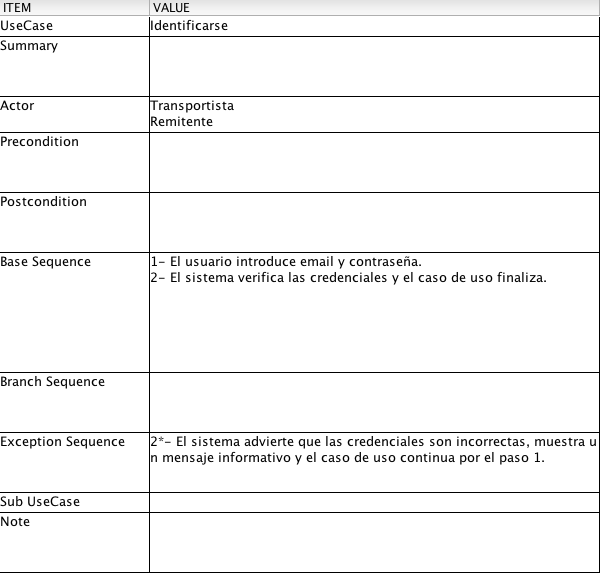
\includegraphics[width=0.75\textwidth]{astah/use_case_identificarse.png}
		\end{figure}

		\begin{figure}[H]
			\centering
				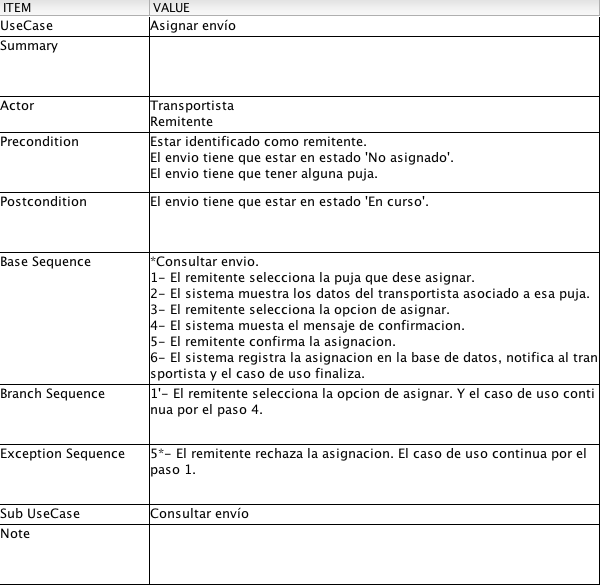
\includegraphics[width=0.75\textwidth]{astah/use_case_asignar_envio.png}
		\end{figure}

		\begin{figure}[H]
			\centering
				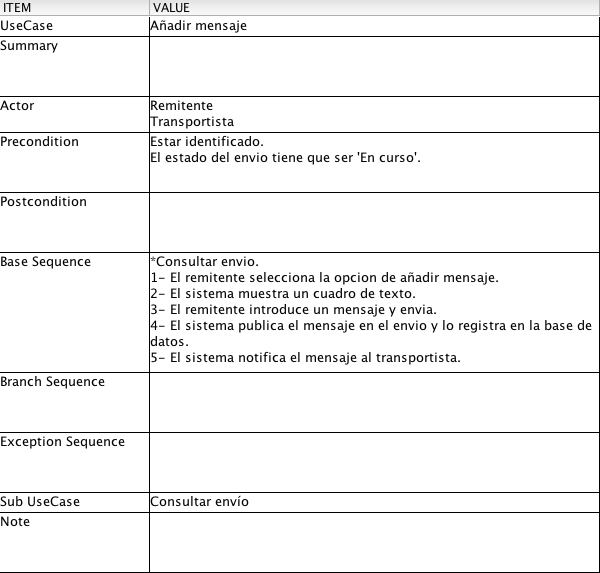
\includegraphics[width=0.75\textwidth]{astah/use_case_anadir_mensaje.png}
		\end{figure}

		\begin{figure}[H]
			\centering
				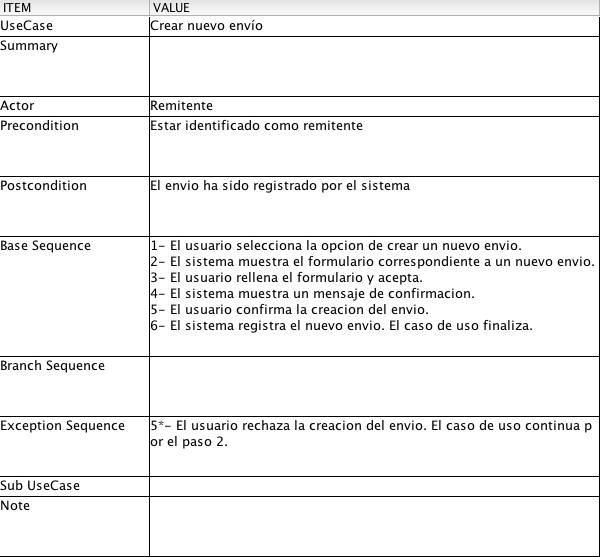
\includegraphics[width=0.75\textwidth]{astah/use_case_crear_envio.png}
		\end{figure}

		\begin{figure}[H]
			\centering
				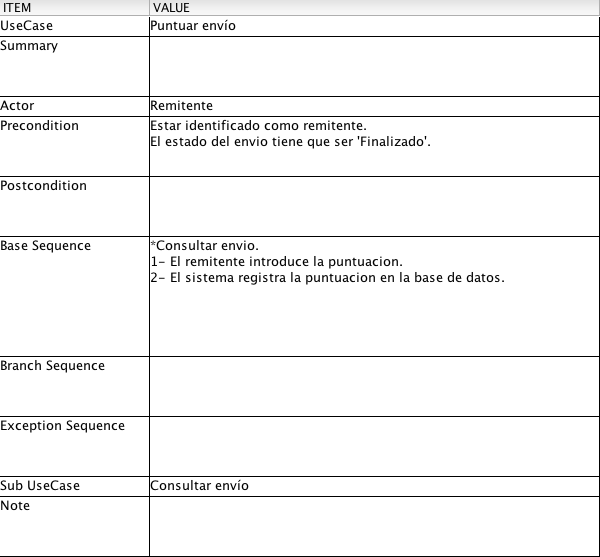
\includegraphics[width=0.75\textwidth]{astah/use_case_puntuar.png}
		\end{figure}

	\section{Modelo del dominio:}

		\begin{figure}[H]
			\centering
				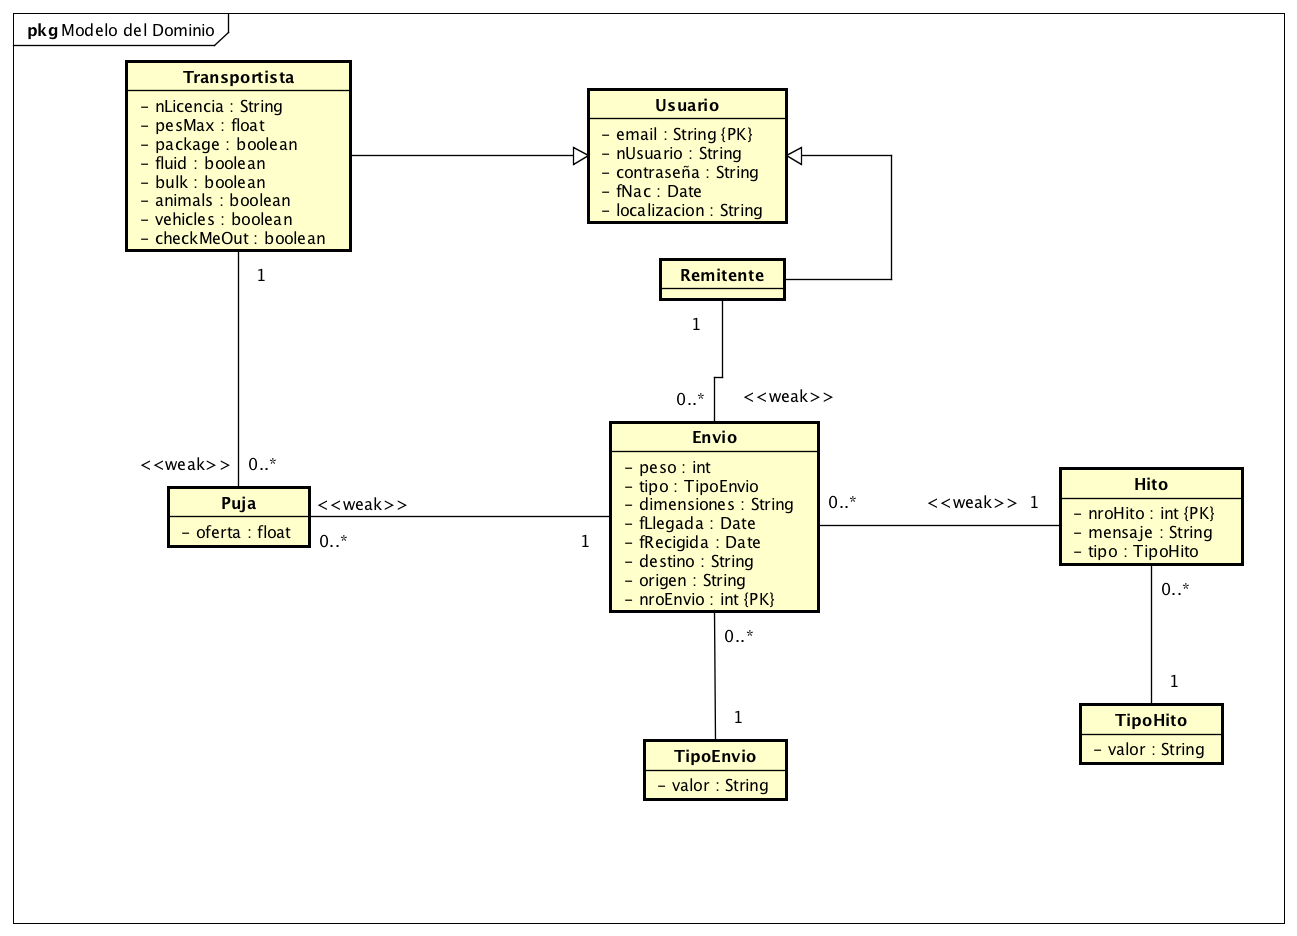
\includegraphics[width=\textwidth]{astah/entidad_relacion.png}
		\end{figure}


	\section{Análisis de los usuarios:}

		\paragraph{}


	\section{Escenarios del sistema futuro:}

		\paragraph{}
		Los escenarios expuestos para el sistema son los siguientes:

		\begin{itemize}
			\item \textbf{Escenario 1:} \\
				Miguel es un camionero que ha oido hablar del sistema, por lo que se decide probar su funcionamiento dado que ha oido muy buenos comentarios sobre él. Nunca antes lo había probado, por lo que crea una cuenta en el sistema indicando que es transportista. Para ello introduce sus datos personales, además del número de licencia de transporte y las características de la mercancía que es capáz de transportar. Una vez creada la cuenta lo siguiente que hace en el sistema es buscar envíos. Para ello introduce su localización actual y el sistema le muestra un listado de las envíos que puede realizar, ofreciendole la posibilidad de pujar por ello. Dado que Miguel quiere probar el sistema se decide a pujar por unos cuantos envíos para probar la utilidad del sistema. Una vez hecho esto, tendrá que esperar hasta que alguna de las pujas sea aceptada.

			\item \textbf{Escenario 2:} \\
				Teresa es una usuaria habitual del sistema, el cuál utiliza para envíar cosas a su familia y amigos dado que le ofrece la facilidad de poder realizar todos los trámites online. Teresa ha decidido mudarse de casa el próximo mes, para lo que utilizará el sistema para trasladar todos sus bienes a su nueva casa. Lo que hará será por tanto crear un nuevo envío para lo cual tendrá que introducir las direcciones de origen y destino así como el tamaño y peso aproximados del envío. Una vez hecho esto espera a que algún transportista ofrezca una puja sobre el envío. En el momento en el que encuentre un precio que esté dispuesta a aceptar y las valoraciones del transportista la convenzan aceptará dicha puja. En este momento será cuando empezará a contactar con él para fijar una fecha para la recogida del envío. Durante todo el proceso de envío tanto el transportista como ella podrá interactuar a través de hitos y comentarios sobre el transporte. Una vez finalizado el envío Teresa podrá introducir una valoración acerca del transportista que después otros usuarios podrán visualizar en el momento de aceptar las pujas.

			\item \textbf{Escenario 3:} \\
				Oscar acaba de comprar una nueva consola a través de internet. La web a través de la cual ha realizado la compra utiliza el sistema para llevar a cabo el transporte, por lo cual le ha enviado un enlace para que pueda monitorizar el proceso. Dado que Oscar todavía no tiene una cuenta en el sistema lo primero que hará será registrarse en el mismo introduciendo sus datos personales, pero omitiendo seleccionar que es un tranportista. Una vez hecho esto podrá consultar su envío a la vez que introducir hitos y comentarios sobre él, que tanto el transportista que lo traslade como el remitente (en este caso la web) podrán visualizar. Una vez finalizado el envío Oscar podrá valorar al transportista.

		\end{itemize}


\end{document}
